\section{Diagramas de conexiones}

El presente esquema muestra la configuración del circuito de potencia diseñado para el ensayo del contactor, integrando una fuente de alimentación variable y los instrumentos de medición necesarios. Este montaje permite regular la tensión aplicada de manera controlada para observar el comportamiento electromagnético del dispositivo bajo distintas condiciones de servicio y verificar sus parámetros nominales de operación.

 \begin{center}
        \begin{figure}[H]
        \centering  
        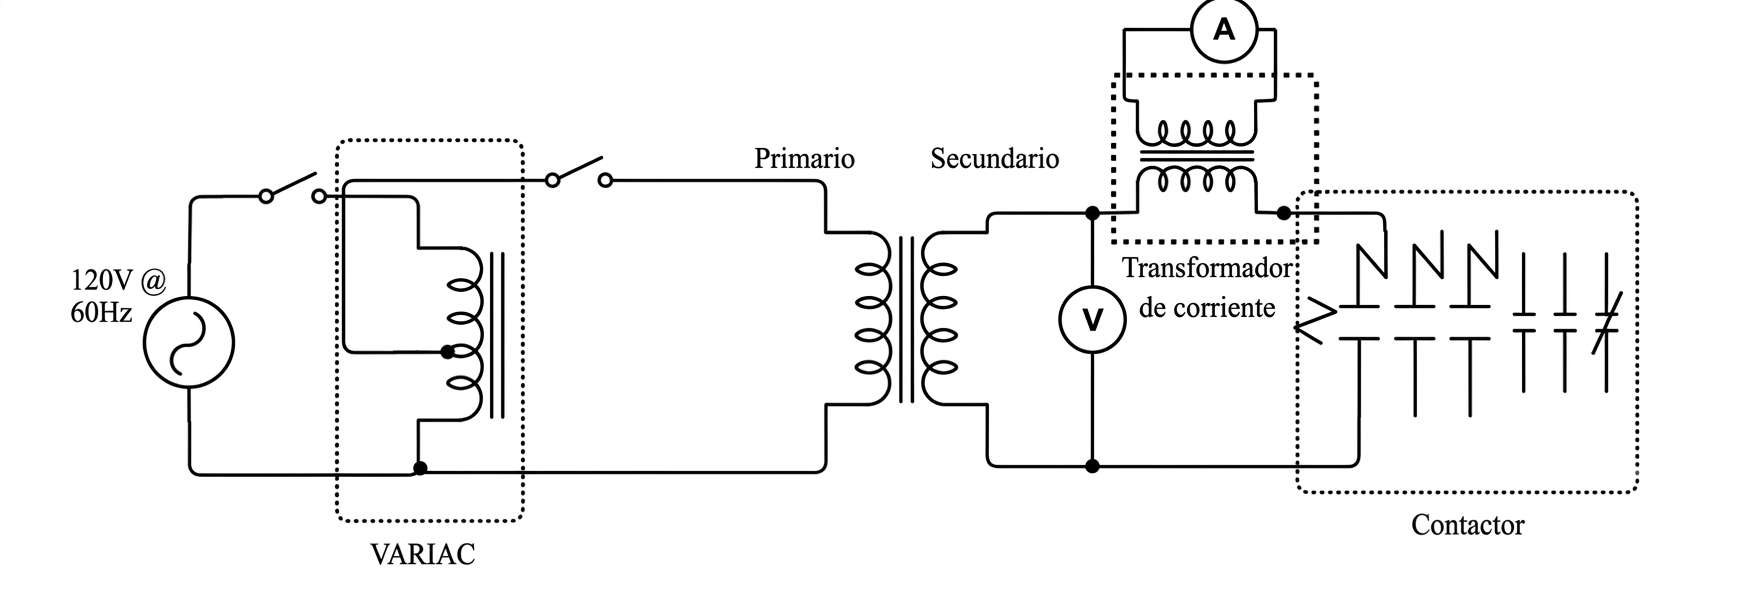
\includegraphics[scale=0.2]{imagenes/1..png}
        \caption{Diagrama circuital para la medicion del contactor}
        \label{Diagrama circuital para la medicion del contactor}
        \end{figure}
    \end{center}

El uso del transformador elevador en este montaje es fundamental debido a una diferencia de niveles de tensión entre la fuente y el equipo de prueba. Dado que el Variac suministra una tensión máxima de 120 V y el contactor bajo estudio requiere una tensión nominal de operación de 220 V, el transformador actúa elevando el voltaje al nivel necesario para alcanzar el estado de activación (cierre) del circuito magnético. Además de adecuar la tensión, este componente proporciona una protección esencial al desacoplar galvánicamente el circuito de prueba de la red eléctrica, incrementando la seguridad durante la manipulación y las mediciones experimentales.

El transformador de corriente (TC) cumple la función esencial de permitir la medición segura de corrientes elevadas, actuando como un dispositivo reductor que transforma una corriente primaria alta en una proporcional menor, apta para ser leída por un amperímetro convencional sin dañarlo. 